\section{Exercise 4}

Let $S_1(t)$ and $S_2(t)$ be two correlated geometric Brownian motions under the risk-neutral measure $\mathbb{Q}$, defined by:

\begin{equation*}
dS_1(t) = r S_1(t)\,dt + \sigma_1 S_1(t)\,dW_1(t), \quad
dS_2(t) = r S_2(t)\,dt + \sigma_2 S_2(t)\,dW_2(t),
\end{equation*}

with initial values $S_1(0) = S_2(0) = S_0$, volatilities $\sigma_1 = 0.4$, $\sigma_2 = 0.15$, constant interest rate $r = 0.01$, and Brownian correlation $\mathbb{E}[dW_1(t)\,dW_2(t)] = \rho\,dt$.

\medskip
Applying the multidimensional Itô lemma to $\log S_i(t)$ leads to:

\begin{equation*}
\log S_i(T) \sim \mathcal{N}\left( \log S_0 + \left(r - \frac{1}{2} \sigma_i^2 \right) T,\; \sigma_i^2 T \right),
\end{equation*}

so the joint vector $(\log S_1(T), \log S_2(T))$ is bivariate normal:

\begin{align*}
X(T) := 
\begin{bmatrix} 
\log S_1(T) \\ 
\log S_2(T) 
\end{bmatrix}
\sim \mathcal{N} \left(
\begin{bmatrix}
\mu_1 \\ 
\mu_2
\end{bmatrix},\;
\begin{bmatrix}
\sigma_1^2 T & \rho \sigma_1 \sigma_2 T \\
\rho \sigma_1 \sigma_2 T & \sigma_2^2 T
\end{bmatrix}
\right),
\end{align*}

where $\mu_i = \log S_0 + \left(r - \frac{1}{2} \sigma_i^2\right)T$.

\medskip
Since $\max(S_1, S_2) = \exp(\max(\log S_1, \log S_2))$, the distribution of the maximum of two lognormal variables can be derived by analyzing the maximum of a bivariate normal vector. The exact distribution and moments of $\max(X_1, X_2)$ are given by Nadarajah and Kotz (2008) \cite{nadarajah2008}, enabling analytical computation of the mean and variance of the transformed maximum.

\bigskip



A Monte Carlo simulation with $N = 10000$ paths and $\text{n\_steps}=100$ was used to approximate the distribution of $\max(S_1(T), S_2(T))$. In the simulation, correlation between the two assets was introduced by expressing the stochastic differentials in terms of two independent Brownian motions. Specifically, the system was modeled as
\begin{align*}
dS_1(t) &= r S_1(t)\,dt + \sigma_1 S_1(t)\,d\tilde{W}_1(t), \\
dS_2(t) &= r S_2(t)\,dt + \rho \sigma_2 S_2(t)\,d\tilde{W}_1(t) + \sqrt{1 - \rho^2}\, \sigma_2 S_2(t)\,d\tilde{W}_2(t),
\end{align*}
where $\tilde{W}_1(t)$ and $\tilde{W}_2(t)$ are independent standard Brownian motions. This construction ensures that the instantaneous correlation between $dS_1(t)$ and $dS_2(t)$ is exactly $\rho$, while preserving the marginal dynamics of geometric Brownian motion for each asset.  Each asset's path was evolved over a single step, and the payoff $\max(S_1(T), S_2(T))$ was computed for each simulation.

\begin{figure}[h!]
\centering
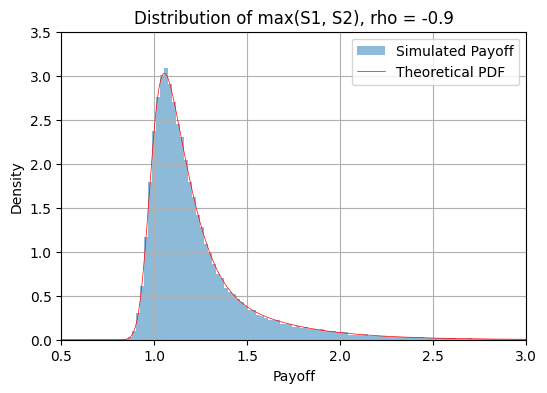
\includegraphics[width=0.49\textwidth]{Exercise_set_02/img/04_rho_neg.png}
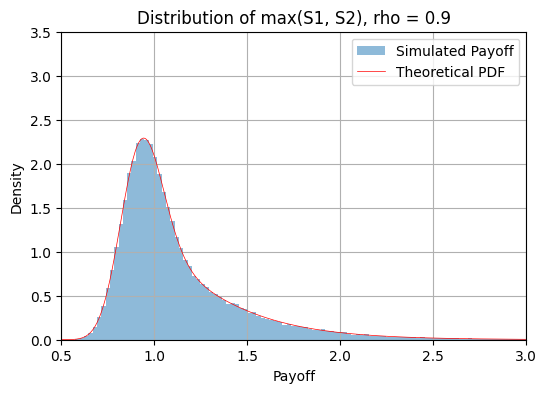
\includegraphics[width=0.49\textwidth]{Exercise_set_02/img/04_rho_pos.png}
\caption{Histogram of simulated $\max(S_1, S_2)$ for $\rho = -0.9$ (left) and $\rho = 0.9$ (right).}
\end{figure}

The sample mean and variance were calculated, and a $95\%$ confidence interval for the expected payoff was constructed using the central limit theorem.

\begin{center}
\begin{tabular}{|c|c|c|c|c|c|}
\hline
$\rho$ & Sample Mean & 95\% CI & Sample Variance & Theor. Mean & Theor. Variance \\
\hline
$-0.9$ & 1.2228 & [1.2210,\;1.2245] & 0.0821 & 1.2219 & 0.0585 \\
\hline
$+0.9$ & 1.1187 & [1.1166,\;1.1208] & 0.1133 & 1.1160 & 0.0852 \\
\hline
\end{tabular}
\end{center}

The simulation confirms that negative correlation increases the spread of possible outcomes, resulting in a higher average maximum. Positive correlation concentrates the joint distribution, lowering both the variance and the expected value of the maximum.

\begin{thebibliography}{1}
\bibitem{nadarajah2008}
S.~Nadarajah and S.~Kotz, ``Exact Distribution of the Max/Min of Two Gaussian Random Variables,'' \emph{IEEE Transactions on VLSI Systems}, vol.~16, no.~2, pp.~210--212, 2008.
\end{thebibliography}
